\documentclass{article}
\usepackage[T1]{fontenc} 
\usepackage[utf8]{inputenc}
\usepackage{graphicx}
\usepackage{float}
\usepackage[czech]{babel}
\usepackage{rotating}

\begin{document}

\begin{titlepage}
    \begin{center}
        
\includegraphics[scale=0.1,keepaspectratio]{fig/logo_cz.png}
        
        \vspace{3cm}
        
        {\Huge \textbf{IDS}}
        
        \vspace{0.25cm}
        
        {\LARGE 2020/2021}
        
        \vspace{2cm}
        \Large
        \begin{tabular}{l l}
                    Karel Norek & xnorek01 \\
    				Martin Kneslík & xknesl02 \\
    	\end{tabular}
    \end{center}

\end{titlepage}

\textbf{\flushleft \LARGE Mafie}

\vspace{0.25cm}

\large Padrino Guiseppe, přítel všech brněnských mafiánů, Vás požádal o vytvoření informačního systému pro organizaci kriminální činnosti a setkání předních brněnských rodin. 
\par V čele každé rodiny je Don (např. Don Calzone, Don Quatro Formagi, Don Funghi, apod.), respektovaná osoba, která organizuje dění rodiny, určena běžnými atributy (jméno, věk, velikost bot, ???). 
\par Samotná famílie pak sestává z řadových členů, kteří nemusí být pokrevně spřízněni a kteří zprostředkovávají veškerou kriminální činnost, jako je odstraňování nevhodných osob, dealování drog, tisknutí falešných peněz, atd., Don si však nikdy nešpiní ruce. 
\par Kriminální činnost probíhá v rámci území, určených gps souřadnicemi, adresou, rozlohou, a mohou být buď řádným rajónem jedné z familií, nebo neutrálním územím, kde může operovat větší počet familií. 
\par Do samotné kriminální činnosti jsou pak zapojeni konkrétní řadoví členové v různých obdobích (tzn. řadový člen může nejprve dealovat drogy a poté přejít na odstraňování osob), přičemž každá činnost je přímo vedena jednou z familií a má různou dobu trvání a tato operace má vždy unikátní jméno. 
\par Do těchto činností může být zapojeno více rodin, to v případě, že dvě rodiny uzavřou alianci, které však nemusí mít dlouhé trvání. 
\par Jednou z hlavních činností jsou pak vraždy, u kterých je vedeno nejen, kde byly provedeny, ale i kdo je provedl a na kom je provedl. Některé z těchto vražd jsou pak objednány samotnými Dony, jiné jsou spontánní, bez bližší objednávky. Cílem vraždy však nikdy není Don. 
\par Systém pravidelně organizuje setkání Donů, kde se probírají výsledky jednotlivých rodin a probíhají buď v rámci neutrálního území, nebo jsou hostěny některou z předních rodin. Systém pak zasílá Donům pozvánky a očekává od nich potvrzení účasti.

\newpage

\begin{figure}[!ht]
    
    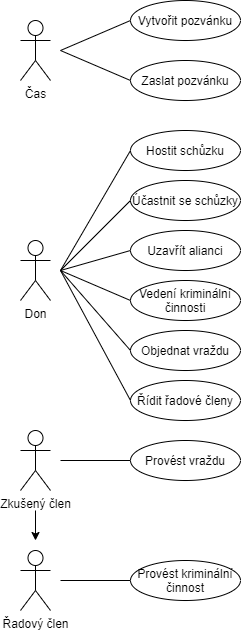
\includegraphics[scale=0.75, keepaspectratio]{fig/USCD.png}
    \caption{Use case diagram pro mafii}
    \label{fig:UCD}
\end{figure}

\newpage

\begin{figure}[!ht]
    \flushleft
    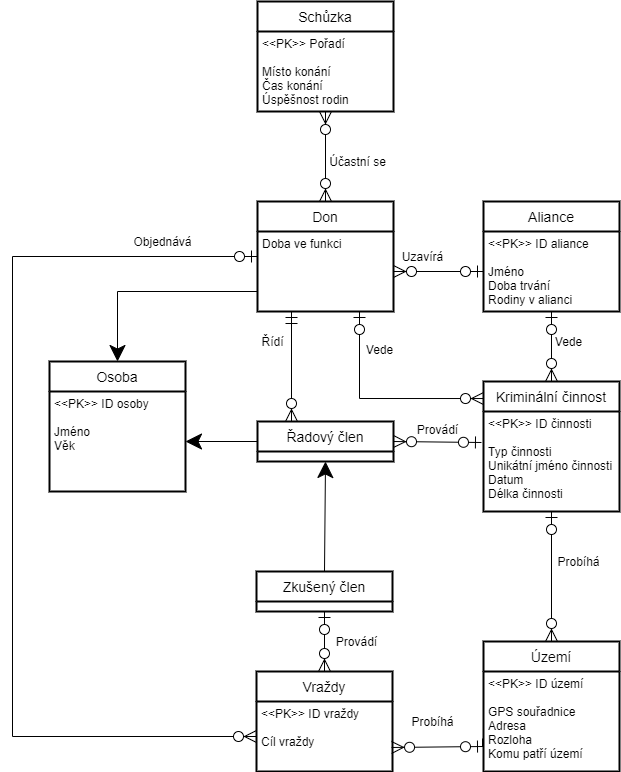
\includegraphics[scale=0.60, keepaspectratio]{fig/ERD.png}
    \caption{ER diagram pro mafii}
    \label{fig:ERD}
\end{figure}

\newpage
\flushleft
\large \textbf{Popis USCD:} \newline
Use case diagram popisuje co může jaký aktér dělat. \newline
\large \textbf{Popis ERD:} \newline
Entita osoba má 2 specializované entity - don a řádový člen. Řadový člen má pak další specializovanou entitu zkušený člen. Don je jediný vůdce rodiny a velí všem svým řádovým členům, kteří slouží právě jednomu donovi a mohou provádět kriminální činnosti na určitém území. Řádový člen může být povýšen na zkušeného člena, který může provádět spontánní, nebo donem objednané vraždy. Don dále může uzavírat alianci s jinými dony. Kriminální činnost může vést samotný don, nebo uzavřená aliance. Don se může účastnit schůzek s dalšími dony. Kriminální činnost probíha na určitém uzemí.

\section*{Implementace}
Na začátku skriptu odstraňujeme pomocí příkazu \texttt{DROP} všechny tabulky, sekvence, materializované pohledy a indexy, které ve skriptu vytváříme.

Dále vytváříme tabulky. Skoro všechny tabulky, které obsahují primární klíč, si automaticky generují primární klíč pomocí \texttt{INT GENERATED AS IDENTITY PRIMARY KEY}. Jediná tabulka, ve které primární klíč negenerujeme, je tabulka \texttt{don}.

V tabulce \texttt{don} generujeme primární klíč pomocí triggeru/sekvence \texttt{don\_id}.
Druhý trigger \texttt{povys\_clena} povýší řadového člena na zkušeného člena po jeho první vykonané vraždě.

Po vytvoření tabulek a triggerů vkládáme do tabulek ukázková data pomocí příkazu \texttt{INSERT}.
Po naplnění databáze lze vykonat ukázky již 2 zmíněných triggerů.

Následují 2 procedury. Procedura \texttt{prumerna\_velikost\_rodiny} vypočítá a vypíše průměrný počet členů v rodině. V proceduře je i ošetřeno dělění nulou - když neexistuje žádný don.
Další procedura \texttt{pocet\_clenu\_cinnosti} vypíše, kolik členů vykonává určitou činnost. V této proceduře používáme kurzor proměnné s datovým typem odkazujícím se na typ sloupce tabulky.

\texttt{EXPLAIN PLAN} provádíme na příkazu, který vypíše počet vražd každého člena.

Materializovaný pohled obsahuje seznam členů v rodině dona Salieriho. 

\end{document}
